%%%%%%%%%%%%%%%%%%%%%%%%%%%%%%%%%%%%%%%%%
% Stylish Article
% LaTeX Template
% Version 2.1 (1/10/15)
%
% This template has been downloaded from:
% http://www.LaTeXTemplates.com
%
% Original author:
% Mathias Legrand (legrand.mathias@gmail.com) 
% With extensive modifications by:
% Vel (vel@latextemplates.com)
%
% License:
% CC BY-NC-SA 3.0 (http://creativecommons.org/licenses/by-nc-sa/3.0/)
%
%%%%%%%%%%%%%%%%%%%%%%%%%%%%%%%%%%%%%%%%%

%-------------------------------------------------------------------------------------
%	PACKAGES 
%-------------------------------------------------------------------------------------

\documentclass[fleqn,11pt]{SelfArx} % Document font size and equations flushed left
\usepackage[francais]{babel} % Specify a different language here - english by default
\usepackage{hyperref}

\setlength{\columnsep}{0.55cm} % Distance between the two columns of text
\setlength{\fboxrule}{0.75pt} % Width of the border around the abstract
\definecolor{color1}{RGB}{0,0,90} % Color of the article title and sections
\definecolor{color2}{RGB}{0,20,20} % Color of the boxes behind the abstract and headings
\usepackage{hyperref} % Required for hyperlinks
\usepackage{xcolor}  
\usepackage{listings}
\usepackage{pdfpages}
\usepackage{amssymb}
%\usepackage[french]{babel}

\usepackage{courier} % Required for the courier font         
\hypersetup{hidelinks,colorlinks,breaklinks=true,urlcolor=blue,citecolor=color1,linkcolor=color1, bookmarksopen=false,pdftitle={Title},pdfauthor={Author}}

\providecommand\phantomsection{}


%--------------------------------------------------------------------------------------
%	CODE INCLUSION CONFIGURATION
%-------------------------------------------------------------------------------------
\usepackage{color}
 
\definecolor{codegreen}{rgb}{0,0.6,0}
\definecolor{codegray}{rgb}{0.5,0.5,0.5}
\definecolor{codepurple}{rgb}{0.58,0,0.82}
\definecolor{backcolour}{rgb}{0.95,0.95,0.92}
 
\lstdefinestyle{mystyle}{
    backgroundcolor=\color{backcolour},   
    commentstyle=\color{codegreen},
    keywordstyle=\color{magenta},
    numberstyle=\tiny\color{codegray},
    stringstyle=\color{codepurple},
    basicstyle=\footnotesize,
    breakatwhitespace=false,         
    breaklines=true,                 
    captionpos=b,                    
    keepspaces=true,                 
    numbers=left,                    
    numbersep=5pt,                  
    showspaces=false,                
    showstringspaces=false,
    showtabs=false,                  
    tabsize=2
}
 
\lstset{style=mystyle}



%-------------------------------------------------------------------------------------
%	INFORMATIONS
%-------------------------------------------------------------------------------------


\JournalInfo{Projet RESYS 2016-2017}
\Archive{Master 2 BIM-BMC, UPMC} 
\PaperTitle{Différenciation des précurseurs hématopoïétiques chez l'embryon}
\Authors{Nathalie Lehmann\textsuperscript{1}, Mariam Sissoko\textsuperscript{1} \\ Enseignants référents: \textbf{Hervé Isambert\textsuperscript{2}, Louis Verny\textsuperscript{2}, Nadir Sella\textsuperscript{2}}}

\affiliation{\textsuperscript{1}\textit{Master 2 Bioinformatique et Modélisation, Université Paris 6, France}}
\affiliation{\textsuperscript{2}\textit{Institut Curie, France}}


\Keywords{Réseaux de régulation -- Facteurs de transcription -- Hématopoïèse} 

\newcommand{\keywordname}{Mots-clés} % Defines the keywords heading name

%--------------------------------------------------------------------------------------
%	ABSTRACT
%--------------------------------------------------------------------------------------

\Abstract{Le but de ce projet de Master 2 de bioinformatique est de reconstruire le réseau de régulation régissant les expressions des facteurs de transcription clés pour la différenciation des précurseurs hématopoïétiques chez l'embryon. Dans cet objectif, nous avons d'abord procédé à un filtrage des données afin de garder les gènes d'intérêt, puis reconstruit des réseaux selon deux méthodes différentes : par clustering hierarchique et via l'algorithme polynomial PC\cite{pc} (\textit{Peter-Clark}). Enfin, en comparant nos résultats avec ceux présents dans la littérature scientifique, nous ferons état d'un modèle graphique simplifié expliquant les mécanismes impliquant la différenciation des cellules primitives en deux lignées distinctes hématopoïétique et endothéliale. Cette reconstruction de réseau a été effectuée à partir de données analysées par \textit{single cell RNA-seq} puis binarisées. }

 



%--------------------------DEBUT-------------------------------------

\begin{document}
\flushbottom % Makes all text pages the same height
\maketitle


\tableofcontents 

\thispagestyle{empty} 


%------------------------------------------------
%--------------INTRO----------------------------------
%------------------------------------------------
\section*{Introduction}
\addcontentsline{toc}{section}{Introduction}
Au cours du développement de l'embryon des Verté-brés, tous les tissus hématopoïétiques successivement actifs (foie, thymus, rate et moelle osseuse) sont colonisés par des cellules souches hématopoïétiques (CSH) d'origine extrinsèque. Le sac vitellin (SV) constitue l'unique exception à cette règle, puisque des CSH s'y développent in situ. Il a été observé que le SV constitue le premier site d'hématopoïèse de l'embryon\cite{Cumano} : c'est le lieu d'apparition des premières cellules sanguines propres à l'embryon. Cependant, de la lignée primitive à l'origine de celles-ci, émerge aussi les premières cellules endothéliales (constituant la paroi interne des vaisseaux sanguins). Dans ces conditions, quels sont les facteurs de transcription suffisants et/ou nécéssaires pour induire cette différenciation de la lignée primitive ?

\par Reconstruire le réseau de régulation contôlant cette différenciation pourrait permet de mieux appréhender les mécanismes de l'hématopoïèse primitive et de la formation des tissus sanguins. Or l'origine de certaines leucémies (ie l'anémie de Fanconi\cite{Fanconi}) reste encore difficile à déterminer, et l'établissement de tels réseaux pourrait alors favoriser la compréhension et l'établissement de protocoles expérimentaux mieux ciblés. 
 
\par Il est important de spécifier que ce projet s'appuie largement sur l'article de Moignard et al., \textit{Decoding the regulatory network of early blood development from single-cell expression measurements}\cite{Moignard}. En effet, les données utilisées pour réaliser ce projet sont similaires à celles utilisées par les auteurs de l'article sus-nommé, et la démarche globale de reconstruction de réseau est relativement semblable, bien qu'allégrement simplifiée. 


%------------------------------------------------
%--------------METHODES----------------------------------
%------------------------------------------------

\section{Données et méthodes}
La reconstruction des voies moléculaires contrôlant le développement embryonique des organes est entrâvé par le manque de méthodes adaptées pour l'étude de phénomènes extrêmement précis, d'autant plus si le matériel disponible est limitant. Les techniques traditionnelles telles que le RNA-seq se révèlent alors insuffisantes. La stratégie que les auteurs de l'article de référence ont choisi est particulièrement pertinente car il s'agit d'une approche combinant le séquençage \textit{single cell} et les analyses computationnelles de reconstruction de réseaux à partir des graphes des états de transition. En effet, le séquençage \textit{single cell} (sc) permet une analyse transcriptomique à l'échelle d'une seule cellule. Grâce au sc-RNAseq, il devient possible d'estimer l'hétérogénéité intra-tumorale, mais aussi d'étudier des stades embryonnaires précoces, ou encore de retracer les lignées cellulaires au cours du développement (source : \href{http://bioinfo-fr.net/single-cell-sequencing?hilite=single+cell+RNA-seq}{bioinfo-fr} )\footnote{http://bioinfo-fr.net}. 


\subsection{Dataset}
Le dataset proposé rassemble les données d'expression binarisées de différents gènes pouvant soit être des facteurs de transcription (33 gènes), soit d'autres gènes marqueurs (spatiaux ou temporels - 9 gènes), ou encore des gènes servant de contrôle (\textit{housekeepers} - 4 gènes). Chaque ligne du dataset correspond au profil d'expression d'une cellule, analysée par sc-RNAseq. Les colonnes, quant à elles, correspondent aux gènes dont l'expression a été quantifiée. Les données étant binaires, le '1' représente un gène exprimé dans la condition correspondante, le '0' un gène non exprimé. Au total, cela fait donc 46 gènes analysés dans 3934 cellules issues d’embryons de souris, prelevées à quatre stades différents du développement embryonnaire précoce. Celles-ci deviendront éventuellement des cellules sanguines (en rouge sur la figure \ref{fig:debut}) ou endothéliales (en violet). Comme indiqué sur la figure \ref{fig:debut}, cinq populations sont analysées :

\begin{itemize}
\item E7.0 (\textit{primitive streak}, PS),
\item E7.5 (\textit{neural plate}, NP) 
\item E7.75 (\textit{head fold}, HF).
\item E8.25, cellules GFP+ (\textit{four somite}, 4SG) cellules sanguines potentielles
\item E8.25, cellules Flk1+GFP− (4SFG−) cellules endothéliales potentielles.
\end{itemize}



\begin{figure}[ht]
\centering
\includegraphics[width=\linewidth]{images/debut2}
\caption{Processus de différenciation de la lignée primitive (PS) en 2 lignées distinctes : endothéliale (4SFG) et hématopoïétique (4SG)}
\label{fig:debut}
\end{figure}

Pour ceux qui souhaiteraient visualiser le cycle de développement embryonnaire murin de manière globale ainsi que les étapes critiques de l'hématopoïèse, les figures récapitulatives \ref{fig:devptCycle} et \ref{fig:devpt} sont accessibles dans la partie annexe. 



\subsection{Filtre des données}
Afin d'obtenir un set de données non biaisées, nous avons choisi d'appliquer un filtre afin d'éliminer les gènes exprimés dans 100\% des cas (codé en Python, on ôte du dataset les colonnes où il n'exsite que des '1'). Les gènes qui disparaissent alors sont référencés ci-dessous, et leur fonction en tant que \textit{housekeepers} a été vérifiée via le site de la \href{https://www.ncbi.nlm.nih.gov/gene}{NCBI}\footnote{https://www.ncbi.nlm.nih.gov/gene} : \textbf{Eif2b1}, \textbf{Mrpl19}, \textbf{Polr2a}, \textbf{Ubc}.

%/ ou via mouse genom database

\subsection{Gènes d'intérêt}
%Expliquer tous les datasets formés : par lignée (fonctionnel) ou par type cellulaire (temporel). 
Une fois le filtre appliqué, il nous a fallu procéder à différents tris des données. 
\subsubsection{Tri par facteur de transcription}
Les 42 gènes restant dans notre dataset n'étant pas tous impliqués directement dans la différenciation cellulaire, nous avons effectué un premier tri où ne sont conservés que les 33 facteurs de transcription. Les gènes marqueurs qui ne se trouvent plus dans le dataset sont les suivants : \textbf{Cdh1}, \textbf{Cdh5}, \textbf{EgfI7}, \textbf{Hbb-bH1}, \textbf{Itga2b} (ou CD41), \textbf{Kdr} (ou Flk1), \textbf{Kit}, \textbf{Pecam1}, \textbf{Procr}. Dans chacun des tris décrits ci-dessous, a été conservé un dataset avec les 42 gènes, et un autre avec les 33 facteurs de transciption afin de permettre d'analyser de façon spécifique toutes les interactions potentielles.
\subsubsection{Tri par stade embryonnaire}
Afin d'étudier les relations au niveau temporel, les données ont été séparées par type cellulaire présent (PS, NP, HF, 4SFG, 4SG). 
\subsubsection{Tri par lignée}
Enfin, une séparation des données au niveau fonctionnel a été effectué. Nous avons alors un dataset pour les gènes préférentiellement exprimés dans la lignée primitive (en bleu sur la figure \ref{fig:filtre33prof}), un autre dont les gènes sont davantage associés à l'hématopoïèse (en rouge) et le dernier pour les gènes impliqués dans la formation de l'endothélium (en rose/violet).

\subsection{Reconstruction de réseaux}
Les réseaux ont été établis en définissant les gènes pour noeuds et les interactions de régulation (activation ou inhibition) comme liens (les données étant des niveaux d'expression binarisés comme décrit ci-dessus). Nous avons choisi d'utiliser deux types d'algorithmes différents.

\subsubsection{Algorithme PC}
Une première démarche pour reconstruire les réseaux est d'appliquer l'algorithme PC\cite{pc} (Peter-Clark). Il s'agit d'un algorithme polynomial pour l'inférence de la structure de graphe. Pour cela, deux choix s'offraient à nous : utiliser le package \textit{pcalg} disponible sur R, ou bien le \href{https://miic.curie.fr}{Miic Web Server}\footnote{https://miic.curie.fr} (\textit{Multivariate Information based Inductive Causation}), outil développé par l'équipe enseignante. La maîtrise facile de l'interface et la diversité des paramètres modifiables pour la manipulation des données ont vite orienté notre choix pour l'utilisation de ce dernier. Nous avons notamment fait usage de l'interface \href{http://cytoscape.org}{Cytoscape}\footnote{http://cytoscape.org} accessible via le Miic Web Server. Miic a pour but de reconstruire des réseaux de causalité, non-causalité, ou bien mixte, entre les variables du dataset qui lui est soumis. Parmi les paramètres par défaut (ceux que nous avons utilisés), on peut noter que les échantillons sont considérés comme indépendants, même pour des conditions expérimentales identiques. Aussi, le réseau est reconstruit par maximum de vraisemblance normalisé (pour des analyses futures, on pourrait faire varier ce critère de complexité, notamment en utilisant la reconstruction basée sur les informations bayésiennes). Enfin, les effets de causes latentes sur les relations entre les noeuds ne sont pas mesurées par défaut mais pourrait également être un critére intéressant pour une analyse plus fine du réseau. 

\begin{figure*}[ht]
\centering
\includegraphics[width=\linewidth]{images/pc}
\caption{Algorithme PC (Spirtes, Glymour, Scheines (1993)}
\label{fig:pcd}
\end{figure*}


\subsubsection{Réseau hierarchique}
Mariam. Code R. Bioconductor. 

%------------------------------------------------
%--------------RESULTATS----------------------------------
%------------------------------------------------

\newpage
\section{Résultats et discussion}
%Faire un choix entre précision (spécificité des données ?) et lisibilité. 
\subsection{Réseaux obtenus}
Face à la diversité des paramètres qui peuvent être modifiés via MIIC (sur l'interface Cytoscape), nous avons choisi de ne nous focaliser que sur un unique paramètre : le seuil de confiance. Ainsi nous avons construit, pour chaque set de données généré, de 2 à 10 réseaux différents, les premiers réseaux ayant un seuil de confiance élevé (par rapport à l'étendue de celui-ci) et les derniers ayant un seuil de confiance plus bas. Le nombre de réseau obtenu est fonction du nombre de gènes compris dans le dataset. Tous les autres paramètres par défaut sont restés inchangés par souci de compréhension. 
% On aurait pu aussi choisir de modifier le confidence cut This step aims at filtering the network according to a confidence ratio, calculated by estimating the probability to discard an edge in more randomization of the input dataset and comparing it to the estimation of the probability in the real dataset. The closer this ratio is to 0, the more trustworthy the edge is.


%Cependant, nous avons testé quelques dataset en modifiant la latence (par défaut : prise en compte) afin de voir si des différences notables quant aux relations entre les noeuds apparaissaient.

Il faut prendre en compte que plus le seuil de confiance est élevé, moins les relations sont nombreuses, donc des gènes disparaissent du réseau ainsi formé. Cependant, ces relations restantes sont d'autant plus fiables. 

\subsubsection{Tri par stade embryonnaire}
Asynchrone, difficulté de recréer un réseau causal. 
Importance des gènes marqueurs en tant qu'inducteur d'un stade embryonnaire... transition assurée par ces gènes ? Ou si gènes présents, suffisants pour passer dans l'état embryonnaire suivant ?


\subsubsection{Tri par lignée}
\begin{figure}[ht]
\centering
\includegraphics[width=\linewidth]{results/bleu}
\caption{Lignée primitive}
\label{fig:PS}
\end{figure}

% devrait pas avoir de Runx1 ou dans l'autre ?
\begin{figure}[ht]
\centering
\includegraphics[width=\linewidth]{results/rouge}
\caption{Lignée hématopïétique}
\label{fig:4SG}
\end{figure}


\begin{figure}[ht]
\centering
\includegraphics[width=\linewidth]{results/violet}
\caption{Lignée endothéliale}
\label{fig:4SFG}
\end{figure}

\begin{figure}[ht]
\centering
\includegraphics[width=\linewidth]{results/filtre33prof}
\caption{Résultats issus de \textit{Verny et al. submitted} (les couleurs correspondent aux lignées décrites dans la figure \ref{fig:debut}).}
\label{fig:filtre33prof}
\end{figure}

\subsection{Similarité des réseaux obtenus avec ceux de la littérature}
\begin{figure*}[ht]
\centering
\includegraphics[width=\linewidth]{results/filtre33}
\caption{Compromis obtenu après de nombreux tests sur les facteurs de transcription uniquement (les couleurs correspondent aux lignées décrites dans la figure \ref{fig:debut}).}
\label{fig:filtre33}
\end{figure*}


\subsection{Vérifications expérimentales}
D'après les données de l'article de référence\cite{Moignard}, on peut observer grâce à la figure \ref{fig:artcile2} présente en annexe, que ...... \\
hub !!! \\ 
rôle central de Sox7 (violet). \\
rôle central (de controle) des cdh1 - cdh5 => nécéssaires pour le changement de transition ? \\
différences 4SG et 4SG33genes. \\


%\begin{figure}[ht]
%\centering
%\includegraphics[width=\linewidth]{images/ikarosNotchGata}
%\caption{ikaros - Notch - Gata}
%\label{fig:ikarosNotchGata}
%\end{figure}

%\begin{figure*}[ht]
%\centering
%\includegraphics[width=\linewidth]{results/arbre1}
%\caption{Arbre obtenu par clustering hierarchique non supervisé - 42 gènes}
%\label{fig:arbre1}
%\end{figure*}

\begin{figure*}[ht]
\centering
\includegraphics[width=\linewidth]{results/arbre33genes2}
\caption{Arbre obtenu par clustering hierarchique non supervisé - 33 gènes}
\label{fig:arbre33}
\end{figure*}



%------------------------------------------------
%--------------CONCLUSION----------------------------------
%------------------------------------------------
\newpage
\section*{Conclusion}
\addcontentsline{toc}{section}{Conclusion}



%------------------------------------------------
\newpage
\phantomsection
\bibliographystyle{unsrt}
\bibliography{sample}

\newpage
\section*{Annexes}

\begin{figure*}[ht]
\centering
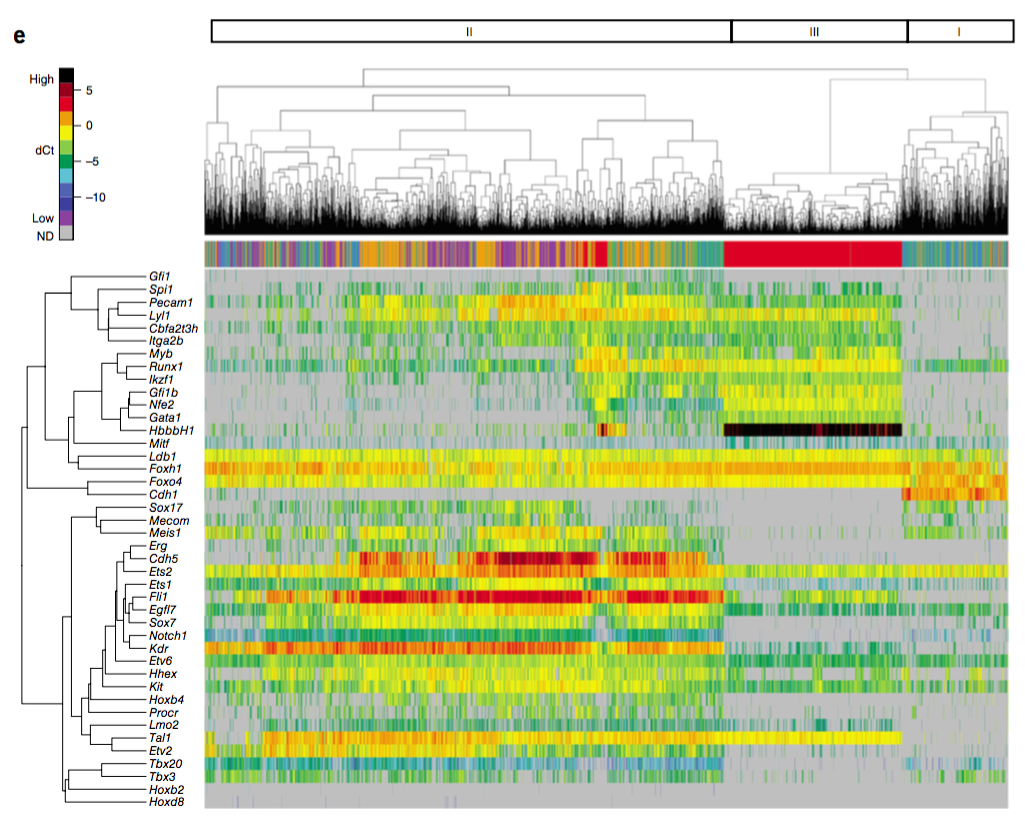
\includegraphics[width=\linewidth]{images/article2}
\caption{Résultats du clustering hierarchique non supervisé issus de \textit{Moignard et al.}. On peut observer le niveau d'expression pour chaque gène dans toutes les cellules. Les colonnes représentent les cellules et les lignes les gènes. Les couleurs correspondent au stade embryonnaire d'où chaque cellule a été extraite.}
\label{fig:artcile2}
\end{figure*}

%\begin{figure*}[ht]
%\centering
%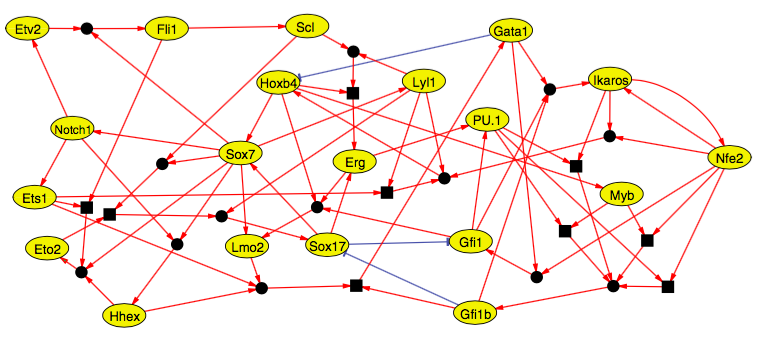
\includegraphics[width=\linewidth]{images/article3}
%\caption{Graphe orienté issus de \textit{Moignard et al.}}
%\label{fig:artcile2}
%\end{figure*}

\begin{figure*}[ht]
\centering
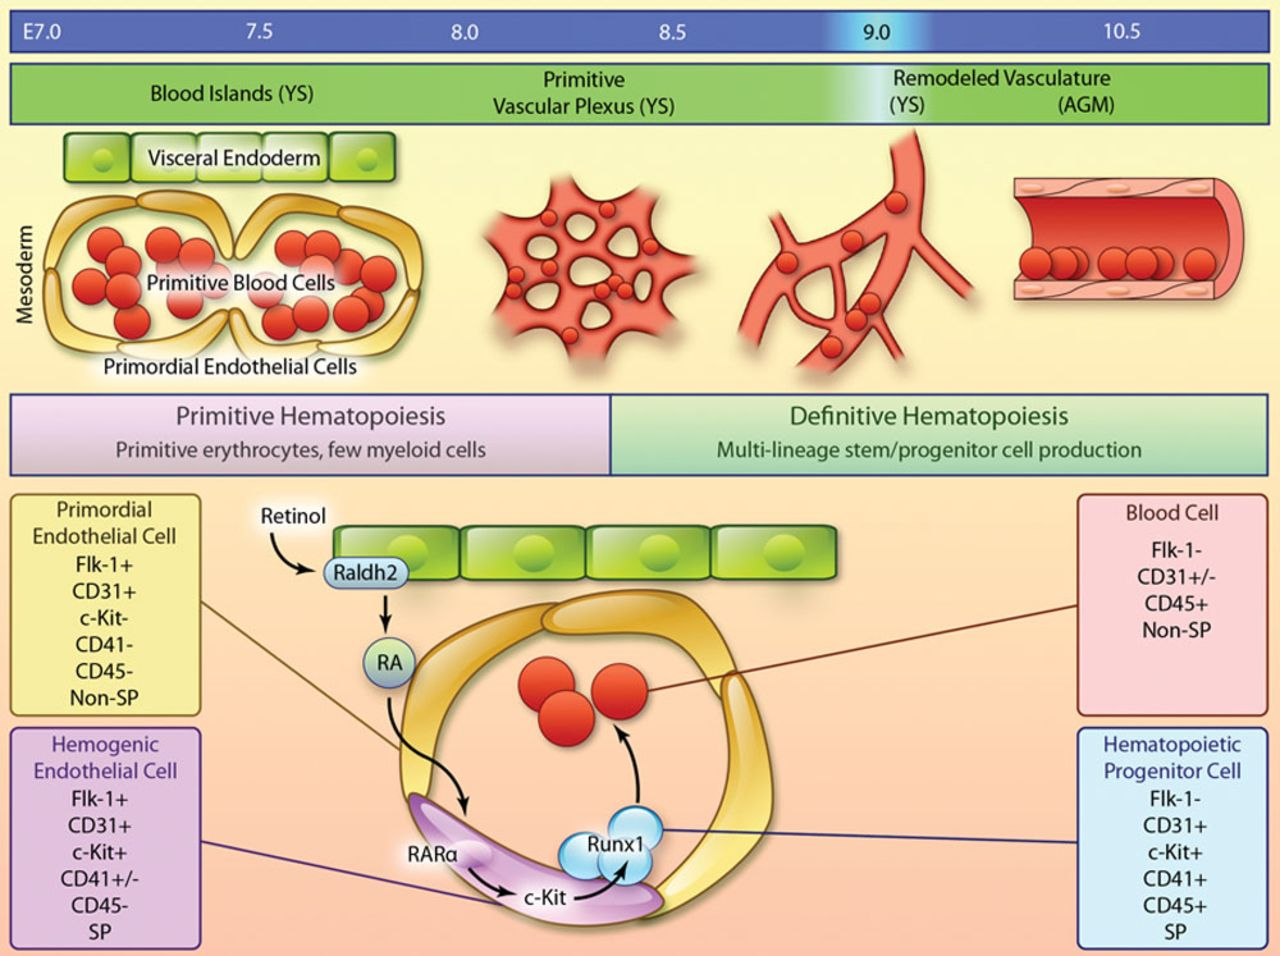
\includegraphics[width=\linewidth]{images/synthese}
\caption{Hematopoiese}
\label{fig:synthese}
\end{figure*}


\begin{figure*}[ht]
\centering
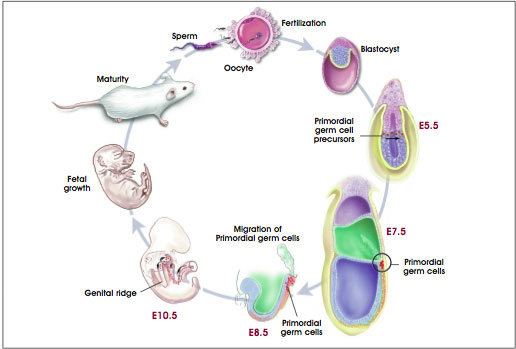
\includegraphics[width=\linewidth]{images/devptCycle}
\caption{Cycle de développement de \textit{Mus musculus}}
\label{fig:devptCycle}
\end{figure*}

\begin{figure*}[ht]
\centering
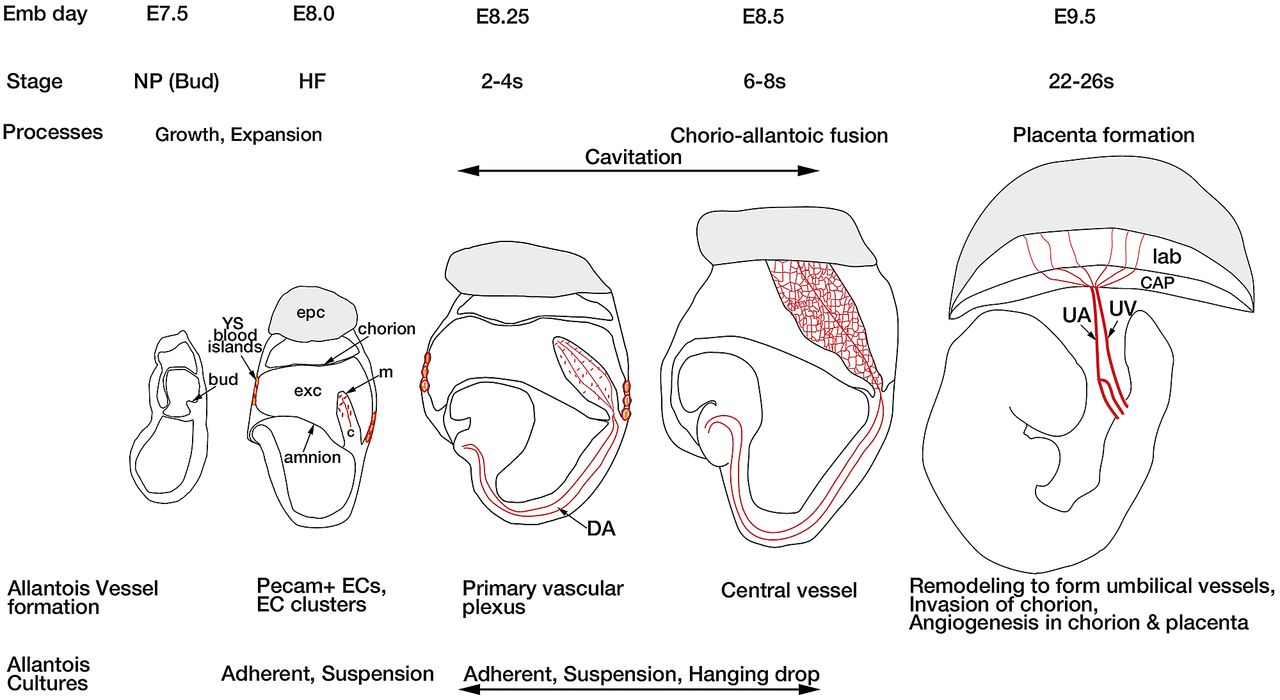
\includegraphics[width=\linewidth]{images/devpt}
\caption{Détails du développement de \textit{Mus musculus}\cite{Gaudin} du stade E7 à E11.5, dans le compartiment extra-embryonnaire (en rouge) et intra-embryonnaire (en jaune). En encart figurent les sites impliqués dans la génération des CSH, c’est-à-dire l’aorte et sa partie ventrale (et les artères omphalomésentérique (OA) et ombilicale (UA)). AGM : aorte-gonades-mésonephros ; FF : foie fœtal ; P-Sp : splanchnopleure para-aortique ; Sp : splanchnopleure ; SV : sac vitellin}
\label{fig:devpt}
\end{figure*}




%\section*{Annexes}

 
%\addcontentsline{toc}{section}{Annexes}
%
%\subsection*{Matériel additionnel} 
%\addcontentsline{toc}{subsection}{Matériel additionnel}
%\subsubsection{Filtres}
%\subsubsection{Fonction de score}

%\begin{figure}[ht]\centering
%\includegraphics[width=\linewidth]{images/poidsScoring}
%\caption{Poids utilisés pour les fonctions de score (utilisés dans RosettaDock\cite{rosettaDOCK}, pour le scoring de haute définition)}
%\label{fig:poidsScoring}
%\end{figure}



%\subsection*{Chronologie du docking}
%\addcontentsline{toc}{subsection}{Chronologie du docking}
%
%\subsection*{Outils de docking}
%\addcontentsline{toc}{subsection}{Outils de docking}


%----------------------------------------------------------------------------------------
%	REFERENCE LIST
%----------------------------------------------------------------------------------------

%----------------------------------------------------------------------------------------

\end{document}






%Articles de réf\cite{Pedotti}
%ref\cite{Rajkannan}
%ref\cite{Sela-Culang}
%ref\cite{Kuroda}
%ref\cite{Krawczyk}
%ref\cite{Abhinandan}
%ref\cite{Gabb}
%\cite{proABC}

%\url{http://www.wikibooks.org}


% Reference to Figure \ref{fig:results}.

%\begin{description}
%\item[Word] Definition
%\item[Concept] Explanation
%\item[Idea] Text
%\end{description}


%\begin{figure*}[ht]\centering % Using \begin{figure*} makes the figure take up the entire width of the page
%\includegraphics[width=\linewidth]{view}
%\caption{Wide Picture}
%\label{fig:view}
%\end{figure*}
%
%\lipsum[4] % Dummy text
%
%\begin{equation}
%\cos^3 \theta =\frac{1}{4}\cos\theta+\frac{3}{4}\cos 3\theta
%\label{eq:refname2}
%\end{equation}
%
%\lipsum[5] % Dummy text
%
%\begin{enumerate}[noitemsep] % [noitemsep] removes whitespace between the items for a compact look
%\item First item in a list
%\item Second item in a list
%\item Third item in a list
%\end{enumerate}
%
%\subsection{Subsection}
%
%\lipsum[6] % Dummy text
%
%\paragraph{Paragraph} \lipsum[7] % Dummy text
%\paragraph{Paragraph} \lipsum[8] % Dummy text
%
%\subsection{Subsection}
%
%\lipsum[9] % Dummy text
%
%\begin{figure}[ht]\centering
%\includegraphics[width=\linewidth]{results}
%\caption{In-text Picture}
%\label{fig:results}
%\end{figure}
%

%\begin{table}[hbt]
%\caption{Table of Grades}
%\centering
%\begin{tabular}{llr}
%\toprule
%\multicolumn{2}{c}{Name} \\
%\cmidrule(r){1-2}
%First name & Last Name & Grade \\
%\midrule
%John & Doe & $7.5$ \\
%Richard & Miles & $2$ \\
%\bottomrule
%\end{tabular}
%\label{tab:label}
%\end{table}

%\footnote{And some mathematics $\cos\pi=-1$ and $\alpha$ in the text.}.
